\section{SingleSource library}\label{section:singl_src}

\subsection{Introduction}

SingleSource library consists of communication channels which implements SC interfaces. There are nine main channels in the library (Fig.~\ref{fig:ss_channels}).

\begin{figure}[!htb]
\centering
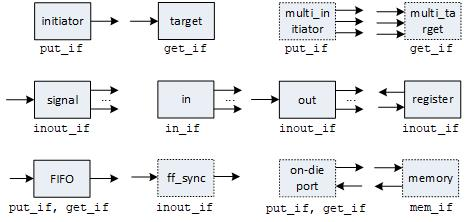
\includegraphics[width=0.9\textwidth]{pics/ss_channels.jpg}
\caption{SingleSource channels}
\label{fig:ss_channels}
\end{figure}

Target and Initiator are intended to connect two SC modules with 1:1 connection. Multi-target and Multi-initiator modules provides 1:N connection to connect multiple SC modules. FIFO is intended to connect two processes in the same module or to serve as a buffer for one process.
On-die port represents any external port to connect SC design to other IPs or fabric. Memory represents any kinds of on-chip SRAM, RF or ROM memory. Register is used to add state for METHOD process. The common use cases of the modules are given in the picture below.

Multi-initiator, multi-target, FF synchronizer, on-die port, and memory are not open-sourced yet.

\begin{figure}[!htb]
\centering
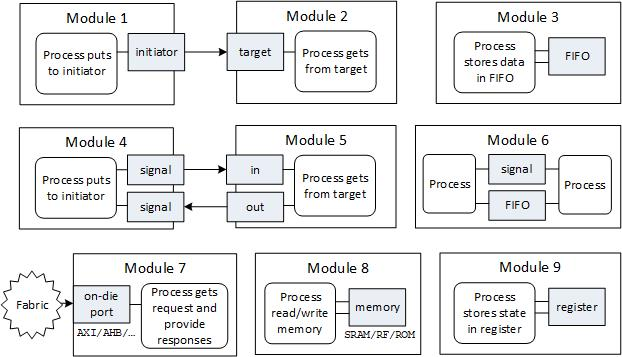
\includegraphics[width=0.9\textwidth]{pics/ss_usage.jpg}
\caption{SingleSource channels usage}
\label{fig:ss_usage}
\end{figure}

The Single Source modules work in two modes: cycle accurate (RTL) and approximate time (TLM). Cycle accurate (RTL) mode intended for hardware synthesis. In RTL mode the modules provide cycle accurate simulation. Approximate time (TLM, Transaction Level Modeling) mode provide fast simulation, intended for virtual prototyping. In TLM mode the modules provide approximate time simulation, there is no clock. Simulation is request-driven, executed in ordered delta-cycles (DC).

\subsubsection{Library files}

\begin{itemize}
\item sct\_common.h -- includes of all library headers and adds namespace \textbf{sct}
\item sct\_ipc\_if.h -- interfaces, general template types and defines
\item sct\_initiator.h -- initiator module
\item sct\_target.h -- target and combinational target modules
\item sct\_multi\_initiator.h -- initiator to connect multiple targets
\item sct\_multi\_target.h -- target to connect multiple initiators
\item sct\_prim\_signal.h -- primitive channel signal implementation with multiple drivers support
\item sct\_signal.h -- signal implementation
\item sct\_ports.h -- input and output ports, sc\_port for target and initiator
\item sct\_fifo.h -- FIFO module
\item sct\_prim\_fifo.h -- primitive channel FIFO implementation, used as base channel in TLM mode
\item sct\_register.h -- register to store METHOD state
\item sct\_clock.h -- clock with enable/disable
\item sct\_clk\_gate\_cell.h -- clock gate and clock gate signal
\item sct\_ff\_sync\_cell.h -- Flip-Flop synchronizer
\item sct\_ff\_sync\_cell.sv -- Flip-Flop synchronizer RTL implementation
\end{itemize}

\subsubsection{Library defines}
{\tt SCT\_TLM\_MODE} could be provided as compile definition: if {\tt SCT\_TLM\_MODE} defined TLM mode is used, RTL mode is used otherwise.

There are multiple options for clock/reset levels:

\begin{itemize}
\item {\tt SCT\_CMN\_TRAITS} -- clock edge and reset level, one of six following options:
\item {\tt SCT\_POSEDGE\_NEGRESET} -- positive clock edge, negative reset level
\item {\tt SCT\_POSEDGE\_POSRESET} -- positive clock edge, positive reset level
\item {\tt SCT\_NEGEDGE\_NEGRESET} -- negative clock edge, negative reset level
\item {\tt SCT\_NEGEDGE\_POSRESET} -- negative clock edge, positive reset level
\item {\tt SCT\_BOTHEDGE\_NEGRESET} -- both clock edges, negative reset level
\item {\tt SCT\_BOTHEDGE\_POSRESE}T -- both clock edges, positive reset level
\end{itemize}

Usually, positive clock edge and negative reset level are used. That is provided by define {\tt  SCT\_CMN\_TRAITS}:
\begin{lstlisting}[style=mycpp]
#ifndef SCT_CMN_TRAITS
  #define SCT_CMN_TRAITS SCT_POSEDGE_NEGRESET
#endif
\end{lstlisting}

If other clock edge/reset levels required, {\tt SCT\_CMN\_TRAITS} value should be provided as compile definition.

There is an {\tt CMakeLists.txt} example where {\tt sct\_def\_traits} target has definitions for TLM mode, negative clock edge and positive reset level:
\begin{lstlisting}[style=mycmake]
add_executable(sct_def_traits sc_main.cpp)
target_compile_definitions(sct_def_traits PUBLIC -DSCT_TLM_MODE)
target_compile_definitions(sct_def_traits PUBLIC -DSCT_CMN_TRAITS=SCT_NEGEDGE_POSRESET)
\end{lstlisting}


\subsection{Library interfaces}\label{section:sct_interfaces}

The interfaces contain non-blocking functions except {\tt b\_put} and {\tt b\_get} which are may-blocking.

Interface {\tt sct\_put\_if}:
\begin{itemize}
\item {\tt bool ready()} -- Return true if it is ready to put request,
\item {\tt void reset\_put()} -- Reset this initiator/FIFO, 
\item {\tt void clear\_put()} -- Clear (remove) request put in this cycle,
\item {\tt bool put(const T\& data)} -- Non-blocking put request into initiator/FIFO if it is ready, return ready to request, 
\item {\tt bool put(const T\& data, sc\_uint<N> mask)} -- Non-blocking put request into initiator/FIFO if it is ready, mask  used to enable/disable put or choose targets in multi-cast put, return ready to request, 
\item {\tt void b\_put(const T\& data)} -- May-blocking put request, could be used in THREAD process only,
\item {\tt void addTo(sc\_sensitive\& s)} -- Add put related signals to process sensitivity,
\item {\tt void addTo(sc\_sensitive* s, sc\_process\_handle* p)} -- Add put related signals to process sensitivity.
\end{itemize}

Interface {\tt sct\_get\_if}:
\begin{itemize}
\item {\tt bool request()} -- Return true if it has request to get,
\item {\tt void reset\_get()} -- Reset this target/FIFO,
\item {\tt void clear\_get()} -- Clear (return back) request got in this cycle,
\item {\tt T peek()} -- Peek request, return current request data, if no request last data returned,
\item {\tt T get()} -- Non-blocking get request and remove it from FIFO/target, return current request data, if no request last data returned,
\item {\tt bool get(T\& data, bool enable)} -- Non-blocking get request and remove it from FIFO/target if {\tt enable} is true, return true if there is a request and {\tt enable} is true,
\item {\tt T b\_get()} -- May-blocking get request, could be used in THREAD process only,
\item {\tt void addTo(sc\_sensitive\& s)} -- Add get related signals to process sensitivity,
\item {\tt void addTo(sc\_sensitive* s, sc\_process\_handle* p)} -- Add get related signals to process sensitivity,
\item {\tt void addPeekTo(sc\_sensitive\& s)} -- Add peek related signal to process sensitivity.
\end{itemize}

Interface {\tt sct\_fifo\_if} inherits sct\_put\_if<T> and sct\_get\_if<T> and has the following additional functions:
\begin{itemize}
\item {\tt unsigned size()} -- FIFO size,
\item {\tt unsigned elem\_num()} -- Number of elements in FIFO, value updated last clock edge for METHOD, last DC for THREAD,
\item {\tt bool almost\_full(const unsigned\& N)} -- Return true if FIFO has (LENGTH-N) elements or more, value updated last clock edge for METHOD, last DC for THREAD,
\item {\tt void clk\_nrst(sc\_in<bool>\& clk\_in, sc\_in<bool>\& nrst\_in)} -- Bind clock and reset to FIFO,
\item {\tt void addTo(sc\_sensitive\& s}) -- Add put and get related signal to process sensitivity,
\item {\tt void addToPut(sc\_sensitive\& s)} -- Add put related signals to process sensitivity,
\item {\tt void addToGet(sc\_sensitive\& s)} -- Add get related signals to process sensitivity.
\end{itemize}

Interface {\tt sct\_in\_if}:
\begin{itemize}
\item {\tt const T\& read()} -- Read from signal/register,
\item {\tt void addTo(sc\_sensitive* s, sc\_process\_handle* p)} -- Add signals to process sensitivity.
\end{itemize}

Interface {\tt sct\_inout\_if}:
\begin{itemize}
\item {\tt const T\& read()} -- Read from signal/register,
\item {\tt void write(const T\& val)} -- Write to signal/register,
\item {\tt void addTo(sc\_sensitive* s, sc\_process\_handle* p)} -- Add signals to process sensitivity.
\end{itemize}

Functions addTo, addToPut, addToGet and addPeekTo are used to add the channel to process sensitivity list. For target and initiator instead addTo {\tt operator <<} can be used. For FIFO instead addToPut and addToGet operator {\tt << fifo.PUT}, {\tt << fifo.GET}, and {\tt << fifo.PEEK} can be used.

\subsection{Processes}\label{section:sct_processes}

SystemC design with single source library can use method and thread processes created with {\tt SC\_METHOD} and {\tt SC\_THREAD} correspondently. It is recommended to use {\tt SCT\_METHOD} and {\tt SCT\_THREAD} macros instead them. Clocked thread process created with {\tt SC\_CTHREAD} is normally not used.

All the channels used in a thread process should use the same clock and edge as the process sensitive. A channel could have different reset or reset level than thread process. If all the channels have different reset or reset level, process reset is specified with third parameter of {\tt SCT\_THREAD} macro.

If a thread process has reset signal, it should have the reset specification with {\tt async\_reset\_signal\_is} or/and {\tt sync\_reset\_signal\_is}. A thread process should be sensitive to all single source channels accessed in its function code. If process is sensitive only to signal and input/output ports, the clock is provided with second parameter of {\tt SCT\_THREAD} macro.

Method process should be sensitive to all single source channels accessed in its function code. Method should not be sensitive to reset, as its provided implicitly through the channels used.

\begin{lstlisting}[style=mycpp]
template <class T>
class MyModule : public sc_module {
   sc_in<bool>      clk{"clk"};
   sct_target<T>    targ{"targ"};
   sct_initiator<T> init{"init"};
   sct_signal<T>    s{"s"};

   explicit MyModule(const sc_module_name& name) : sc_module(name) {
        SC_THREAD(thrdProc1); 
        sensitive << targ;                     // Clock and reset taken from targ
        async_reset_signal_is(nrst, 0);        // Reset specification required

        SCT_THREAD(thrdProc2, clk, nrst);      // Clock and reset explicitly provided
        sensitive << s;
        async_reset_signal_is(nrst, 0);        // Reset specification required 

        SC_METHOD(methProc); 
        sensitive << init;                     // No reset in sensitivity
   }
};
\end{lstlisting}

If any process sensitive to a channel which is not read inside or not sensitive to a channel which is read inside, error reported by ICSC. The error is reported for single channels and for vector/array of channels, no individual channels in vector/array are considered here.


\subsection{Target and Initiator}\label{section:sct_targ_init}

Target and Initiator are channels intended to connect two user defined modules. Initiator implements {\tt sct\_put\_if} interface and could be used in one METHOD or THREAD process to put requests. Target implements {\tt sct\_get\_if} interface and could be used in one METHOD or THREAD process to get requests which put by the connected Initiator.

To connect two modules, Target placed in one modules, Initiator in another one. Target and Initiator should be connected to clock and reset with {\tt clk\_nrst()} function. Target and Initiator are connected to each other with method {\tt bind()}, called in their common parent module constructor. Both Target and Initiator have method {\tt bind()}, any of them can be called.

\begin{figure}[!htb]
\centering
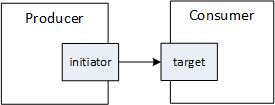
\includegraphics[width=0.5\textwidth]{pics/ss_targ_init.jpg}
\caption{Target and Initiator channels}
\label{fig:ss_usage}
\end{figure}

\begin{lstlisting}[style=mycpp]
struct Producer : public sc_module {
    sc_in<bool>         clk{"clk"};
    sc_in<bool>         nrst{"nrst"};
    sct_initiator<T>    init{"init"};
    explicit Producer (const sc_module_name& name) : sc_module(name) {
        init.clk_nrst(clk, nrst);
    } 
}
struct Consumer : public sc_module {
    sc_in<bool>         clk{"clk"};
    sc_in<bool>         nrst{"nrst"};
    sct_target<T>       targ{"targ"};
    explicit Consumer (const sc_module_name& name) : sc_module(name) {
        targ.clk_nrst(clk, nrst);
    } 
}
struct Top: public sc_module {
    Producer prod{"prod"};
    Consumer cons{"cons"};
    explicit Top(const sc_module_name& name) : sc_module(name) {
        prod.clk(clk); prod.nrst(nrst);
        cons.clk(clk); cons.nrst(nrst);
        // Call bind() method of initiator or bind() method of target
        prod.init.bind(cons.targ);  
    }
}
\end{lstlisting}

Target and Initiator have the same template parameters:
\begin{lstlisting}[style=mycpp]
template<
    class T,                              // Payload data type 
    class TRAITS = SCT_CMN_TRAITS,        // Clock edge and reset level traits
    bool TLM_MODE = SCT_CMN_TLM_MODE>     // RTL (0) or TLM (1) mode
class sct_initiator {};

template<
    class T,                              // Payload data type 
    class TRAITS = SCT_CMN_TRAITS,        // Clock edge and reset level traits
    bool TLM_MODE = SCT_CMN_TLM_MODE>     // RTL (0) or TLM (1) mode
class sct_target {};
\end{lstlisting}

Target and Initiator constructor parameters:
\begin{lstlisting}[style=mycpp]
sct_target(const sc_module_name& name, 
           bool sync_ = 0,                // Is register required to pipeline request 
           bool always_ready_ = 0);       // Is always ready to get request

sct_initiator(const sc_module_name& name,
           bool sync_ = 0);               // Is register required to pipeline request  
\end{lstlisting}

\subsection{Target and initiator usage}\label{section:sct_targ_init_usage}

Target and initiator can be used in SystemC method process. The method process should be created with {\tt SC\_METHOD} or {\tt SCT\_METHOD}  macro in the module constructor. The method process should have sensitivity list with all the targets/initiators accessed in the process function.

\begin{lstlisting}[style=mycpp]
// Initiator and target in method process example
struct Producer : public sc_module {
    sct_initiator<T>         init{"init"};
    explicit Producer (const sc_module_name& name) : sc_module(name) {
       SC_METHOD(initProc); 
       sensitive << init;
    } 
    void initProc {
       // Put data into init
    }
}

struct Consumer : public sc_module {
    sct_target<T>       targ{"targ"};   
    explicit Consumer (const sc_module_name& name) : sc_module(name) {
       SC_METHOD(targProc); 
       sensitive << targ;
    } 
    void targProc{
       // Get data from targ
    }
}
\end{lstlisting}

Target and initiator can be used in clocked thread process. Clocked thread process should be created with {\tt SC\_THREAD} or {\tt SCT\_THREAD} macro, but not with {\tt SC\_CTHREAD}. The thread process should have sensitivity list with all the targets/initiators accessed in the process function as for method process. If the thread process has reset signal, it should have the reset specification with {\tt async\_reset\_signal\_is} or/and {\tt sync\_reset\_signal\_is}.

\begin{lstlisting}[style=mycpp]
// Initiator and target in thread process example
struct Producer : public sc_module {
    sct_initiator<T>         init{"init"};
    explicit Producer (const sc_module_name& name) : sc_module(name) {
       SC_THREAD(initProc); 
       sensitive << init;
       async_reset_signal_is(nrst, 0);
    } 
    void initProc {
       // Reset init to set default values
       wait();
       while(true) {
          // Put data into init 
          wait();
       }
    }
}

struct Consumer : public sc_module {
    sct_target<T>       targ{"targ"};   
    explicit Consumer (const sc_module_name& name) : sc_module(name) {
       SC_THREAD(targProc); 
       sensitive << targ;
       async_reset_signal_is(nrst, 0);
    } 
    void targProc{
       // Reset init to set default values
       wait();
       while(true) {
          // Get data from targ
          wait();
       }
    }
}
\end{lstlisting}

There are three kinds of connections which could be organized:
\begin{itemize}
\item Combinational,
\item Buffered,
\item Buffered with FIFO.
\end{itemize}

\subsubsection{Combinational connection}

In combinational connection request part of connection contains {\tt core\_req} and {\tt core\_data} signals, which could be used directly or through the pipelining register (specified with second parameter of Target/Initiator constructor). There is no back-pressure signal, so Target process should be always ready to get request. Initiator process does not need to check ready to put request (method {\tt ready()} always returns true).

\begin{figure}[!htb]
\centering
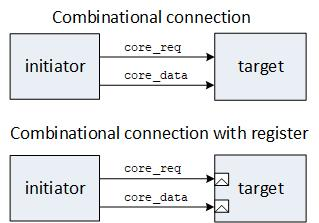
\includegraphics[width=0.5\textwidth]{pics/ss_comb_conn.jpg}
\caption{Combinational connection}
\label{fig:ss_usage}
\end{figure}

Combinational connection is provided with last parameter of {\tt sct\_target<>} constructor or with using special target class {\tt sct\_comb\_target<>}.

In combinational connection put data into Initiator can be done without checking if the Initiator is ready.

\begin{lstlisting}[style=mycpp]
// Initiator and always ready target in method process example
struct Producer : public sc_module {
    sct_initiator<T>         init{"init"};
    explicit Producer (const sc_module_name& name) : sc_module(name) {
       SC_METHOD(initProc); sensitive << init;
    } 
    void initProc {
       T val = getSomeValue();          // Put at every path, reset is not required 
       init.put(val);                   // Do not check ready() as Target is always ready
    }						   
}

struct Consumer : public sc_module {
    // Combinational target
    sct_comb_target<T>       targ{"targ"};   
    explicit Consumer (const sc_module_name& name) : sc_module(name) {
       SC_METHOD(targProc); sensitive << targ;
    } 
    void targProc{
       T val;
       if (targ.get(val)) {             // Get at every path, reset is not required
           doSomething(val);        
       }
    }
}
\end{lstlisting}

In thread process it needs to reset Initiator and Target in the reset section.
\begin{lstlisting}[style=mycpp]
// Initiator and always ready target in thread process example
struct Producer : public sc_module {
    sct_initiator<T>         init{"init"};
    explicit Producer (const sc_module_name& name) : sc_module(name) {
       SC_THREAD(initProc); sensitive << init;
       async_reset_signal_is(nrst, 0);
    } 
    void initProc {
       init.reset_put();                 // Reset is required in thread process
       wait();
       while(true) {
          T val = getSomeValue();        // Put every cycle
          init.put(val);                 // Do not check ready() as Target is always ready
          wait();				   
       }
    }
}

struct Consumer : public sc_module {
    sct_comb_target<T>       targ{"targ"};   
    explicit Consumer (const sc_module_name& name) : sc_module(name) {
       SC_THREAD(targProc); sensitive << targ;
       async_reset_signal_is(nrst, 0);
    } 
    void targProc{
       targ.reset_get();                 // Reset is required in thread process
       wait();
       while(true) {
          if (targ.request()) {         
              doSomething(targ.get());
          }
          wait();
       }
    }
}
\end{lstlisting}
Using Target and Initiator in method and thread process looks very similar. In the next sections examples using method and thread process will be mixed.

\subsubsection{Buffered connection}

In buffered connection {\tt core\_ready} signal is used as backpressure when Target is not ready to get request. This connection called buffered as it has the buffer register inside Target or Initiator to store one request if Target is not ready. This kind of connection is the most common and used as default one.

Request part of the connection contains {\tt core\_req} and {\tt core\_data} signals, which could be used directly or through the pipelining register (specified with second parameter of Target/Initiator constructor). The pipelining register is additional to the buffer register. Response part contains {\tt core\_ready} signal which is passed through register to avoid combinational loop. If target process is method this register explicitly added, if it is thread this register is implicitly provided by the process.

\begin{figure}[!htb]
\centering
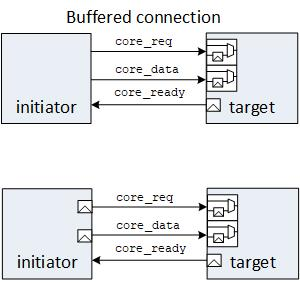
\includegraphics[width=0.5\textwidth]{pics/ss_buff_conn.jpg}
\caption{Buffered connection}
\label{fig:ss_usage}
\end{figure}

\begin{lstlisting}[style=mycpp]
struct Producer : public sc_module {
    sct_initiator<T>         init{"init"};
    explicit Producer (const sc_module_name& name) : sc_module(name) {
       SC_METHOD(initProc); sensitive << init;
    } 
    void initProc {
       init.reset_put();                  // Reset required as put done at some paths only  
       if (init.ready()) {                // Check ready required, target can be not ready 
          init.put(getSomeValue());
       }
    }
}

struct Consumer : public sc_module {
    sct_target<T>       targ{"targ"};
    explicit Consumer (const sc_module_name& name) : sc_module(name) {
       SC_THREAD(targProc); sensitive << targ;
       async_reset_signal_is(nrst, 0);
    } 
    void targProc {
       targ.reset_get();
       wait();
       while(true) {
          if (targ.request()) {      
              doSomething(targ.get()); 
          }
          wait(); 
       }
    }
}
\end{lstlisting}


\subsubsection{Buffered connection with FIFO}

The buffered connection with FIFO provides additional buffer to store requests until their processed by the target process. FIFO can be added to Target with {\tt add\_fifo()} method:

\begin{lstlisting}[style=mycpp]
template<unsigned LENGTH>                  // FIFO size (maximal number of elements)
void add_fifo(bool sync_valid = 0,         // Is register required to pipeline request
          bool sync_ready = 0,             // Is register required to pipeline ready 
          bool init_buffer = 0);           // Initialize all the elements with zeros 
                                           // First element to get is always initialized
\end{lstlisting}

\begin{figure}[!htb]
\centering
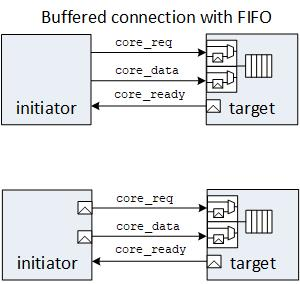
\includegraphics[width=0.5\textwidth]{pics/ss_buff_fifo_conn.jpg}
\caption{Buffered connection with FIFO}
\label{fig:ss_usage}
\end{figure}

\begin{lstlisting}[style=mycpp]
template<class T>
struct A : public sc_module {
    sct_target<T>       run{"run"}; 
    explicit A(const sc_module_name& name) : sc_module(name) {
        run.clk_nrst(clk, nrst);
        run.template add_fifo<2>(1, 1);  // Add FIFO with 2 element and registers 
    }
}
\end{lstlisting}

\subsubsection{Initiator-to-Target Protocol}

The discussed protocol considers buffered connection w/o FIFO. Request is taken by Target when {\tt core\_req} and {\tt core\_ready} both are high. Target can return it to the target process immediately or store the request in the buffer. Initiator sets new request when the previous one has been taken.

The first diagram below represents Target and Initiators accessed in thread processes. The second diagram represents Target and Initiators accessed in method processes.

\begin{figure}[!htb]
\centering
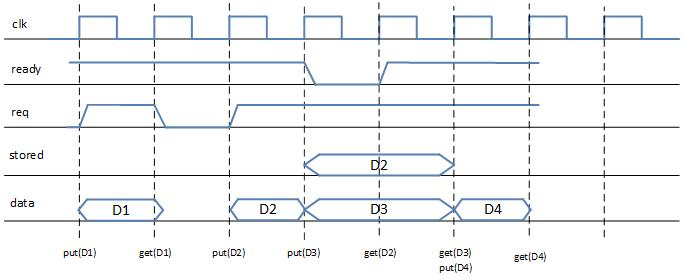
\includegraphics[width=0.98\textwidth]{pics/ss_prot_tt.jpg}
\caption{Initiator-to-Target in THREAD processes}
\label{fig:ss_usage}
\end{figure}

\begin{figure}[!htb]
\centering
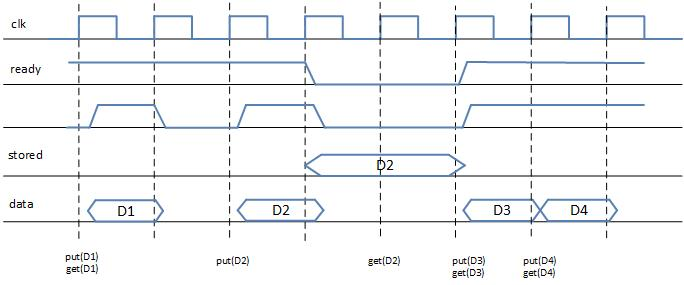
\includegraphics[width=0.98\textwidth]{pics/ss_prot_mm.jpg}
\caption{Initiator-to-Target in METHOD processes}
\label{fig:ss_usage}
\end{figure}

\subsection{Signal and ports}\label{section:sct_signal}
Signal can be used for inter-process communication between processes in the same module. For communication between processes in different modules input/output ports are used together with signal.

\begin{figure}[!htb]
\centering
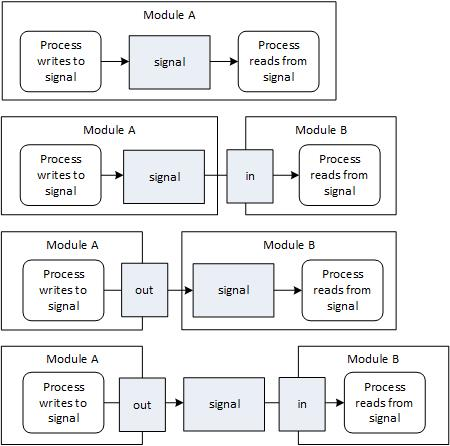
\includegraphics[width=0.7\textwidth]{pics/ss_sig_usage.jpg}
\caption{Signal and ports}
\label{fig:ss_usage}
\end{figure}

Signal and output port implement {\tt sct\_inout\_if}, and can be written by one process. Signal, input and output ports implement {\tt sct\_in\_if}, and can be read by one or mode processes.

\begin{lstlisting}[style=mycpp]
template<
    class T, bool TLM_MODE = SCT_CMN_TLM_MODE>
class sct_signal {};
template<
    class T, bool TLM_MODE = SCT_CMN_TLM_MODE>
class sct_in {};
template<
    class T, bool TLM_MODE = SCT_CMN_TLM_MODE>
class sct_out {};
\end{lstlisting}

Using signal and input/output ports in thread process requires to have clock/reset for these channels which provided with {\tt SCT\_THREAD} macro:
\begin{lstlisting}[style=mycpp]
// Used if the process sensitive to signals/ports only  
SCT_THREAD(proc, clk, rst);  
// Used if the process sensitive to signals/ports and other channels
SCT_THREAD(proc, clk);       
\end{lstlisting}

In this example sigThread sensitive to signals only:
\begin{lstlisting}[style=mycpp]
sct_signal<T>   s{"s"};
MyModule(const sc_module_name& name) : sc_module(name) {  
   // Clock edge/reset level taken from SCT_CMN_TRAITS
   SCT_THREAD(sigThread, clk, nrst); 
   // Only signal `s` is read inside the process
   sensitive << s;                   
   async_reset_signal_is(nrst, 0);
}
\end{lstlisting}

{\tt sc\_vector} of {\tt sct\_signal}, {\tt sct\_in} and {\tt sct\_out} supported. Binding of while vector to another vector is supported.
\begin{lstlisting}[style=mycpp]
class A : public sc_module {
    sc_vector<sct_out<T>>      resp{"resp", 3};
};
class Top {
    A   a{"a"};
    sc_vector<sct_signal<T>>   resp{"resp", 3};

    Top (const sc_module_name& name) : sc_module(name) {        
        a.resp(resp);                  // All vector elements bound
    }
}
\end{lstlisting}

In RTL mode {\tt sct\_signal} is based on {\tt sc\_signal}, {\tt sct\_in}/{\tt sct\_out} are based on {\tt sc\_in}/{\tt sc\_out}.


\subsection{FIFO}\label{section:sct_fifo}

The FIFO can be used for inter-process communication between processes in the same module and for storing requests inside one process. Also the FIFO could be used inside of Target as an extended buffer.

\begin{figure}[!htb]
\centering
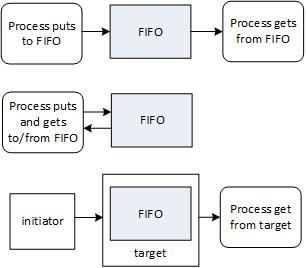
\includegraphics[width=0.5\textwidth]{pics/ss_fifo.jpg}
\caption{FIFO}
\label{fig:ss_fifo}
\end{figure}

FIFO implements {\tt sct\_fifo\_if} interface. FIFO has size template parameter which is a positive number.
\begin{lstlisting}[style=mycpp]
template<
    class T, 
    unsigned LENGTH,                      // Size (maximal number of elements)
    class TRAITS = SCT_CMN_TRAITS,        // Clock edge and reset level traits
    bool TLM_MODE = SCT_CMN_TLM_MODE>     // RTL (0) or TLM (1) mode
>
class sct_fifo {};
\end{lstlisting}

FIFO can have combinational or registered request ({\tt core\_req} and {\tt core\_data}) and response ({\tt core\_ready}) kind which specified in constructor parameters.
\begin{lstlisting}[style=mycpp]
sct_fifo(const sc_module_name& name, 
         bool sync_valid = 0,            // Request path has synchronous register 
         bool sync_ready = 0,            // Response path has synchronous register  
         bool use_elem_num = 0,          // Element number/Almost full or empty used 
         bool init_buffer = 0)           // Initialize all buffer elements with zeros in reset
                                         // First element to get is always initialized to zero 
\end{lstlisting}

\subsubsection{Minimal FIFO size required}

Minimal FIFO size required given in Table.~\ref{tab:fifo_size}.
\begin{table}
\begin{tabular}{|l|l|l|l|l|}
\hline
Initiator process & Target process & sync\_valid & sync\_ready & Minimal FIFO size \\
\hline
method & method & 0 & 0 & 1 \\
method & method & 0 & 1 & 1 \\
method & method & 1 & 0 & 1 \\
method & method & 1 & 1 & 2 \\
method & thread & 0 & 0 & 1 \\
method & thread & 0 & 1 & 2 \\
method & thread & 1 & 0 & 2 \\
method & thread & 1 & 1 & 3 \\
thread & method & 0 & 0 & 1 \\
thread & method & 0 & 1 & 2 \\
thread & method & 1 & 0 & 2 \\
thread & method & 1 & 1 & 3 \\
thread & thread & 0 & 0 & 2 \\
thread & thread & 0 & 1 & 3 \\
thread & thread & 1 & 0 & 3 \\
thread & thread & 1 & 1 & 4 \\
\hline
\end{tabular}
\caption{Minimal FIFO size}
\label{tab:fifo_size}
\end{table}

\subsubsection{Using FIFO for inter-process communication}

FIFO could be used for processes communication instead of set of signals. FIFO has only one writer and one reader process, in comparison with {\tt sct\_signal} which could be read in multiple processes. For 1:N communication array or {\tt sc\_vector} of FIFOs could be used.

\begin{lstlisting}[style=mycpp]
struct Top : public sc_module {
    sct_fifo<T, 2>      fifo{"fifo", 1};     // Pipelining register for request
    explicit Top(const sc_module_name& name) : sc_module(name) {
        fifo.clk_nrst(clk, nrst);
        SC_THREAD(producerProc); 
        sensitive << fifo.PUT;               // Process puts to FIFO
        async_reset_signal_is(nrst, 0);
        SC_METHOD(consumerProc); 
        sensitive << fifo.GET;               // Process gets from FIFO   
    } 
}

void producerProc() {
    fifo.reset_put();
    wait();
    while (true) {
       if (fifo.ready()) {                  // If FIFO is ready put next value
          fifo.put(getSomeVal());
       }
       wait();
    }
}
void consumerProc() {
    fifo.reset_get();
    T val;
    if (fifo.get(val)) {
       doSomething(val);
    }
}
\end{lstlisting}

\subsubsection{One process stores requests in FIFO}

One process stores requests in FIFO example.
\begin{lstlisting}[style=mycpp]
struct Top : public sc_module {
    sc_in<bool>         clk{"clk"};
    sc_in<bool>         nrst{"nrst"};
    sct_fifo<T, 5>      fifo{"fifo"};
    explicit Top(const sc_module_name& name) : sc_module(name) {
        fifo.clk_nrst(clk, nrst);
        SC_THREAD(storeProc); 
        sensitive << fifo;                 // Process puts and gets to FIFO
        async_reset_signal_is(nrst, 0);
    }
}

void storeProc() {
    fifo.reset();
    wait();
    while (true) {
       if (fifo.ready()) {
          fifo.put(getSomeValue());
       }
       wait(); 
       if (fifo.request()) {
          doSomething(fifo.get());
       }
    }
}
\end{lstlisting}


\subsection{Register}

Register is used to add state for METHOD process. Register is written in one method process and could be read in the same or other method process(es). Register is normally added to sensitivity list of process where it is read. Register can be read in thread process.

\begin{figure}[!htb]
\centering
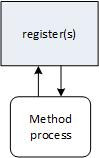
\includegraphics[width=0.17\textwidth]{pics/ss_reg.jpg}
\caption{Register}
\label{fig:ss_reg}
\end{figure}

Register has the same template parameters as Target/Initiator:
\begin{lstlisting}[style=mycpp]
template<
    class T,                            // Payload data type 
    class TRAITS = SCT_CMN_TRAITS,      // Clock edge and reset level traits
    bool TLM_MODE = SCT_CMN_TLM_MODE>   // RTL (0) or TLM (1) mode
class sct_register {};
\end{lstlisting}

Register has the following methods:

\begin{lstlisting}[style=mycpp]
// Reset register, set it value to stored at last clock edge
void reset();
// Write new value to register
void write(const T& data);
// Read value stored at last clock edge
T read();
// To skip using read()
operator T ();
\end{lstlisting}

Register can initiate a new request. That means an output request can depend on register state.

\begin{lstlisting}[style=mycpp]
sct_target<T>       targ{"targ"};
sct_register<T>     cntr{"cntr"};
explicit A(const sc_module_name& name) : sc_module(name) {
    targ.clk_nrst(clk, nrst);
    cntr.clk_nrst(clk, nrst);
    SC_METHOD(checkProc); sensitive << targ << cntr;
}

void checkProc() {
    cntr.reset();
    // Register accumulates received data up to N
    if (cntr.read() > N) {
        cntr.write(0); 
    } else 
    if (targ.get(data)) {
        cntr.write(cntr.read()+data); 
    }
}
\end{lstlisting}


Read register in thread process should be done carefully. If register value is checked to generate an output or change a state, it could lead to incorrect behavior in TLM, if there is no other activation source for the process. 
\begin{lstlisting}[style=mycpp]
sct_register<T>     cntr{"cntr"};
sct_initiator<T>    init{"init"};
explicit A(const sc_module_name& name) : sc_module(name) {
    cntr.clk_nrst(clk, nrst);
    init.clk_nrst(clk, nrst);
    SCT_THREAD(cntrProc); sensitive << cntr << init;
    async_reset_signal_is(nrst, 0);
    // cntr is assigned in some method process 
}

// Probably incorrect version
void cntrProc() {
    init.reset_put();
    wait();
    while (true) {
        if (cntr.read() > 10) {          // In TLM mode no process activation 
           init.b_put(cntr.read());      // until cntr value changed
        }
        wait();
    }
}

// Correct version
void cntrProc() {
    init.reset_put();
    T lastCntr = 0;
    wait();
    while (true) {
        // Request sent only when cntr value changed  
        if (cntr.read() > 10 && cntr.read() != lastCntr) {
           lastCntr = cntr.read();       
           init.b_put(cntr.read());     
        }
        wait();
    }
}
\end{lstlisting}
The same problem is actual for {\tt sct\_signal}.

\subsection{Clock, clock gate and clock gate signal}

{\tt sct\_clock<>} is implementation of clock source (generator) like {\tt sc\_clock} with enable/disable control.

\begin{lstlisting}[style=mycpp]
    /// Enable clock activity, clock is enabled after construction 
    void enable();   
    /// Disable clock activity, can be called at elaboration phase to disable
    /// clock at simulation phase start
    void disable();    
    /// Register clock gate signals/ports to control clock activity.
    /// If any of the signals/ports is high, then clock is enabled
    void register_cg_enable(sc_signal_inout_if<bool>& enable);
    /// Get clock period    
    const sc_time& period() const;
\end{lstlisting}

Clock gate cell {\tt sct\_clock\_gate\_cell} and clock signal {\tt sct\_clk\_signal} should be used together to connect clock input to gated clock source. {\tt sct\_clk\_signal} is special signal without DC delay in written value becomes readable.

\begin{figure}[!htb]
\centering
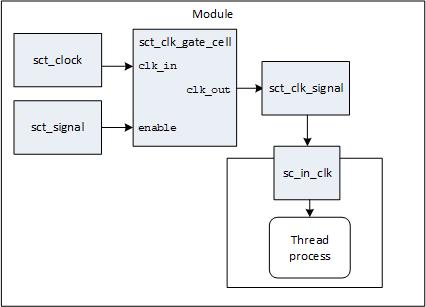
\includegraphics[width=0.7\textwidth]{pics/ss_clock.jpg}
\caption{Clock and clock gate}
\label{fig:ss_clock}
\end{figure}

The code example illustrates using  {\tt sct\_clock\_gate\_cell} and  {\tt sct\_clk\_signal}.

\begin{lstlisting}[style=mycpp]
SC_MODULE(A) {
    sc_in_clk               SC_NAMED(clk);
    sc_in<bool>             SC_NAMED(nrst); 
    sc_in<bool>             SC_NAMED(clk_enbl);
    sct_clk_signal          SC_NAMED(clk_out);
    sct::sct_clk_gate_cell  SC_NAMED(clk_gate);
    sc_in<bool>             SC_NAMED(clk_in);

    explicit A(const sc_module_name& name) : sc_module(name) {
        clk_gate.clk_in(clk);        // Clock input
        clk_gate.enable(clk_enbl);   // Gate clock input 
        clk_gate.clk_out(clk_out);   // Gated clock output    
        clk_in(clk_out);
        
        SCT_THREAD(thrdProc, clk_in, nrst);   // Use clock input bound to gated clock
        async_reset_signal_is(nrst1, 0);
}};
\end{lstlisting}

Clock gate cells can be sequentially connected to each other, gated clock output of one cell bound to clock input of anther cell.

In TLM mode is all thread processes are created with {\tt SC\_THREAD}/{\tt SCT\_THREAD} macros, clock source(s) can be disabled. Disabling {\tt sct\_clock} allows to speed simulation:
\begin{lstlisting}[style=mycpp]
sct_clock<>     clk{"clk", 1, SC_NS};
explicit A(const sc_module_name& name) : sc_module(name) {
    if (SCT_CMN_TLM_MODE) {
         clk.disable();
    }
}
\end{lstlisting}

\subsection{Reset}

\subsubsection{Reset section}

In thread process reset logic initializes registers, local variables and output signals. This logic should be placed in reset section (code scope before first {\tt wait()}).
\begin{lstlisting}[style=mycpp]
sct_out<T> o{"o"};
sct_signal<T> s{"s"};
void thrdProc() {
    // Reset section
    int a = 0;                  // Local variable
    s = 0;                      // Register 
    o = 0;                      // Output 
    wait();
    while (true) {
        ...
        wait(); 
    } 
}
\end{lstlisting}

In method process initialization logic initializes local variables and output signals. This logic is normally be placed in the beginning of the process.
\begin{lstlisting}[style=mycpp]
sct_out<T> o{"o"};
void methdProc() {
    // Initialization section
    int a = 0;                  // Local variable
    o = 0;                      // Output 
    ...
    a = i + 1;
    if (s) o = a;
}
\end{lstlisting}

Initialization logic in method process could be merged with its behavior logic based on inputs and registers. Such code style can have better simulation performance.
\begin{lstlisting}[style=mycpp]
sct_in<T> i{"i"};
sct_out<T> o{"o"};
void methdProc() {
    int a = i+1;                // Local variable
    o = a ? s : 0;              // Output 
    ...
}
\end{lstlisting}

The communication channels also need to be reset with specified {\tt reset()}, {\tt reset\_get()} and {\tt reset\_put()} methods. In thread process every channel used in this process should be initialized in the reset section.
\begin{lstlisting}[style=mycpp]
sct_initiator<T>  init{"init"};
sct_target<T>     targ{"targ"};
sct_fifo<T, 2>    fifo{"fifo"};
void thrdProc() {
    init.reset();
    targ.reset();
    fifo.reset_put();           // If FIFO used for put
    fifo.reset_get();           // If FIFO used for get
    fifo.reset();               // If FIFO used for get and put both
    wait();
    while (true) {
        ...
        wait(); 
    } 
}
\end{lstlisting}

In method process every channel used in this process is initialized in the beginning of the process or assigned at all execution path in the process code. Having no explicit reset for registers, signals, output ports and synchronizers can improve simulation performance.
\begin{lstlisting}[style=mycpp]
sct_initiator<T>  init{"init"};
sct_target<T>     targ{"targ"};
sct_register<T>   reg1{"reg1"};
sct_register<T>   reg2{"reg2"};
void methProc() {
    init.reset();
    reg1.reset();        
    T val = targ.get();  // targ is accessed at all path, no reset required
    if (val > 0) {
        reg1 = val;      // reg1 accessed at some paths only, reset required
        init.put(val);   // init accessed at some paths only, reset required
    }
    reg2 = val + 1;      // reg2 is accessed at all path, no reset required 
}
\end{lstlisting}


\subsubsection{Reset control}
Reset signal can be asserted/de-asserted in TB and DUT processes as well. To have the same simulation time in RTL and TLM modes it needs to follow the rules given in this section.

If reset control thread is in TB, it could control reset based on time period and be non-sensitive to any channels. In this case such a thread should be {\tt SC\_CTHREAD} in RTL mode and {\tt SC\_THREAD} in TLM mode. To avoid extra activation in TLM mode, this thread should wait for a specified time instead of clock events.
\begin{lstlisting}[style=mycpp]
SC_MODULE(A) {
   SC_CTOR(A) {
       // Thread not sensitive to anything
       #ifdef SCT_TLM_MODE
          SC_THREAD(resetProc);
       #else
          SC_CTHREAD(resetProc, clk_in.pos());
       #endif
   }
   #define rstWait(N) if (SCT_CMN_TLM_MODE) wait(N, SC_NS); else wait(N);
   void resetProc() {
        nrst = 0; 
        rstWait(3);
        cout << sc_time_stamp() << " " << sc_delta_count() << " de-assert reset\n";
        nrst = 1; 
        rstWait(5);
        ...
   } 
};
\end{lstlisting}

If reset control thread is sensitive to any channels, it should be {\tt SCT\_THREAD} and have {\tt dont\_initialize()} in RTL mode. Such a thread can also be a normal test thread which provides stimulus and checks results:
\begin{lstlisting}[style=mycpp]
SC_MODULE(A) {
   SC_CTOR(A) {
       // Thread sensitive to SS channels
        SCT_THREAD(resetProc, clk);
        #ifndef SCT_TLM_MODE
            dont_initialize();
        #endif
        sensitive << s;
   }
   sct_signal<unsigned>  s{"s"};
   void resetProc() {
        nrst = 0; 
        while (s.read() < 3) {s = s.read()+1; wait();}
        cout << sc_time_stamp() << " " << sc_delta_count() << " de-assert reset\n";
        nrst = 1; 
   }
\end{lstlisting}

\subsubsection{Specify clock edge and reset level}

Clock edge and reset level normally are the same for the design. To update them for whole design {\tt SCT\_CMN\_TRAITS} should be defined:
\begin{lstlisting}[style=mycpp]
#define SCT_CMN_TRAITS SCT_NEGEDGE_POSRESET   // Set negative edge and positive reset level
\end{lstlisting}

To specify clock edge and reset level for individual library modules, template parameters should be used, for example:
\begin{lstlisting}[style=mycpp]
sct_target<T, SCT_NEGEDGE_POSRESET>       run{"run"};
sct_initiator<T, SCT_POSEDGE_NEGRESET>    resp{"resp"};
\end{lstlisting}


\subsection{Array of SingleSource channels}

Array of SingleSource channels can be implemented with {\tt sc\_vector}. First parameter of {\tt sc\_vector} is name, second parameter is number of elements (should be a compile time constant). To provide additional parameters to single source channels, it needs to use lambda function as third parameter of {\tt sc\_vector}.

\begin{lstlisting}[style=mycpp]
static const unsigned N = 16;
using T = sc_uint<16>;
sc_vector<sct_target<T>>       targ{"targ", N};    // Two parameters 
sc_vector<sct_initiator<T>>    init{"init", N,     // Three parameters
   [](const char* name, size_t i) {                // Lambda function         
        return sc_new<sct_initiator<T>>(name, 1);  // Initiator with sync register
   }}; 
\end{lstlisting}

\subsection{Target and initiator in top module}

Target and Initiator can be instantiated in top module to be connected to the correspondent modules in testbench. Such top module is synthesizable with input/output ports for the Target/Initiator instances.

Top module can contain Target which is not always ready and has no synchronous register. Top module can contain initiator which has no synchronous register. Top module cannot contain MultiTarget or MultiInitiator. Vector ({\tt sc\_vector}) of Target/Initiator in top module is supported.

\begin{figure}[!htb]
\centering
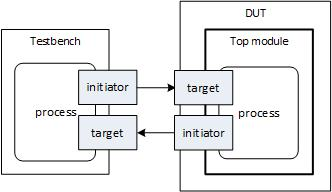
\includegraphics[width=0.55\textwidth]{pics/ss_top_mod.jpg}
\caption{Target and initiator in top module}
\label{fig:ss_top_mod}
\end{figure}

To connect testbench Target/Initiator to the correspondent top module Initiator/Target normal {\tt bind()} function is used always except multi-language simulation. For multi-language simulation if DUT is in SystemVerilog and testbench is in SystemC language, the simulation tool generates a special SystemC wrapper for DUT top module. To connect this wrapper to SystemC testbench {\tt SCT\_BIND\_CHANNEL} macro should be used. {\tt  SCT\_BIND\_CHANNEL} macro cannot be applied to Target/Initiator with record type.

\begin{lstlisting}[style=mycpp]
// Include DUT module generated wrapper or SystemC header 
#ifdef RTL_SIM
    #include "DUT.h"          // Multi-language simulation, include generated wrapper
#else 
    #include "MyDut.h"        // SystemC simulation and synthesis, include designed header
#endif

template<class T>
class MyModule : public sc_module {
   DUT                       dut{"dut"}; 
   sct_target<T>             targ{"targ"};
   SC_CTOR(MyModule) {
       // Bind targ to init in dut module 
       #ifdef RTL_SIM
           SCT_BIND_CHANNEL(dut, init, targ);         // Multi-language simulation
       #else 
           targ.bind(dut.init);                       // SystemC simulation and synthesis
       #endif
   }
}
\end{lstlisting}

\subsection{Array of Target/Initiator in top module}

Array of Targets/Initiators supported in any module including top module. Instead of C++ array {\tt sc\_vector} should be used (C++ array is not supported). To bind the Targets/Initiators {\tt SCT\_BIND\_CHANNEL} macro with 4 parameters is provided.

\begin{lstlisting}[style=mycpp]
// Include DUT module generated wrapper or SystemC header 
#ifdef RTL_SIM
    #include "DUT.h"         // Multi-language simulation, include generated wrapper
#else 
    #include "MyDut.h"       // SystemC simulation and synthesis, include designed header
#endif

template<class T, unsigned N>
class MyModule : public sc_module {
   DUT              dut{"dut"}; 
   sc_vector<sct_target<T>>    targ{"targ", N};
   SC_CTOR(MyModule) {
       // Bind all elements of targ to elements of init in dut module 
       #ifdef RTL_SIM
           SCT_BIND_CHANNEL(dut, init, targ, N);   // Multi-language simulation
       #else 
           for (unsigned i = 0; i != N; ++i)  
               targ[i].bind(dut.init[i]);          // SystemC simulation and synthesis
       #endif
   }
}
\end{lstlisting}

\subsection{Hierarchical connection of Target and Initiator}

Target and Initiator can be connected through module hierarchy from child module up to parent module. To do that {\tt sc\_port} of Initiator/Target in parent module should be used. Ports ({\tt sc\_port}) of Target/Initiator contain pointer to them. To bind Initiator to Target through ports it needs to use {\tt get\_instance()} method which provides Target/Initiator from its port.

\begin{figure}[!htb]
\centering
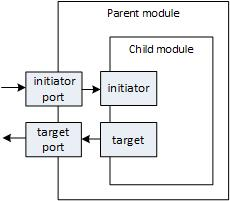
\includegraphics[width=0.4\textwidth]{pics/ss_parent_mod.jpg}
\caption{Target and initiator ports}
\label{fig:ss_parent_mod}
\end{figure}

\begin{lstlisting}[style=mycpp]
template<class T>
struct Child : public sc_module {
    sct_target<T>       run{"run"};
    sct_initiator<T>    resp{"resp"};
};

template<class T>
struct Parent: public sc_module  {
   // Target/initiator ports
    sc_port<sct_target<T>>       run;   
    sc_port<sct_initiator<T>>    resp;   

    Child<T>                     child{"child"};
  
    explicit Parent(const sc_module_name& name) : sc_module(name) {
        // Bind ports to child module target/initiator
        run(child.run);      
        resp(child.resp);
    }
};

struct Top: public sc_module  {
    Parent<T>                    parent{"parent"};
  
    explicit Parent(const sc_module_name& name) : sc_module(name) {
        // Bind child target/initiator to eahc other through parent ports
        // get_instance() provides Initiator from its sc_port   
        parent.run->bind(parent.resp->get_instance());   
    }
};
\end{lstlisting}
Process which calls Target/Initiator functions should be in the module where Target/Initiator declared. If a process calls Target/Initiator through its port ({\tt sc\_port<sct\_target>/sc\_port<sct\_initiator>}) the process module and target initiator module should be synthesized in the same parent module.

\subsection{Cycle accurate and SingleSource code mix}

Conventional cycle accurate SystemC modules can be mixed with single source modules without limitations. {\tt sct\_clock} should be used instead of normal {\tt sc\_clock}.

Cycle accurate threads created with {\tt SC\_CTHREAD} macro are activated by clock event. Such processes can use SingleSource channels to communicate to each other and SingleSource threads created with {\tt SCT\_THREAD} macro. Cycle accurate processes should be sensitive to all the SingleSource channels used inside.

\begin{lstlisting}[style=mycpp]
template<class T>
class MyModule : sc_module {
    sct_target<T>       in{"in"};
    sct_signal<T>       s{"s"};
    sct_fifo<T, 2>      fifo{"fifo"};

    MyModule(const sc_module_name& name) : sc_module(name) {
        SC_CTHREAD(threadProc, clk);
        sensitive << in << fifo.PUT << s;    // sensitivity to all used channels
        async_reset_signal_is(nrst, 0);
    }
    void threadProc() {
        in.reset_get();
        fifo.reset_put();
        wait();
        while (true) {
            if (in.request()) {
                fifo.put(s.read()); 
                in.get();
            }
            wait();
        }
    }
}
\end{lstlisting}

Instead of {\tt SC\_CTHREAD} special {\tt SCT\_CTHREAD} macro could be used. {\tt SCT\_CTHREAD} supports clock edge with third parameter:

\begin{lstlisting}[style=mycpp]
SCT_CTHREAD(proc, clk, clk_edge);   // clk_edge 0 -- negedge, 1 -- posedge, 2 -- both edges
SCT_CTHREAD(proc, clk);             // clk_edge is SCT_CMN_TRAITS::CLOCK
\end{lstlisting}

\subsection{Record as data type in SingleSource channels}

Record is supported as data type in all SingleSource channels. The record should comply SystemC requirements for records used in signal/port: the record should have default constructor w/o parameters, {\tt operator==()}, {\tt operator<<(std::ostream)} and {\tt sc\_trace()} implemented.

\begin{lstlisting}[style=mycpp]
struct Rec_t {
    bool enable;
    sc_uint<16> addr;
    // Default constructor
    Rec_t() : enable(false), addr(0) {}
    // Another constructor, optional
    Rec_t(bool enable_, sc_uint<16> addr_) : enable(enable_), addr(addr_) {}    
    bool operator == (const Rec_t& other) const {
        return (enable == other.enable && addr == other.addr && indx == other.indx);
    }
};
namespace std {
inline ::std::ostream& operator << (::std::ostream& os, const Rec_t& r) {
    os << r.enable << r.addr << r.indx; return os;}
}
namespace sc_core {
void sc_trace(sc_trace_file* , const Rec_t& , const std::string&) {}
}
...
sct_target<Rec_t>   run{"run"};
void methProc() {
   run.reset_get();
   if (run.request()) {
      Rec_t data = run.get();   // Get record fields from target
   }
}
\end{lstlisting}

See more examples at {\tt design/tests/records}

\begin{lstlisting}[style=mycpp]
\end{lstlisting}
